\documentclass{standalone}
\usepackage{tikz}
\usetikzlibrary{patterns, positioning}
\usepackage[sfdefault]{ClearSans} %% option 'sfdefault' activates Clear Sans as the default text font
\usepackage[T1]{fontenc}

\begin{document}
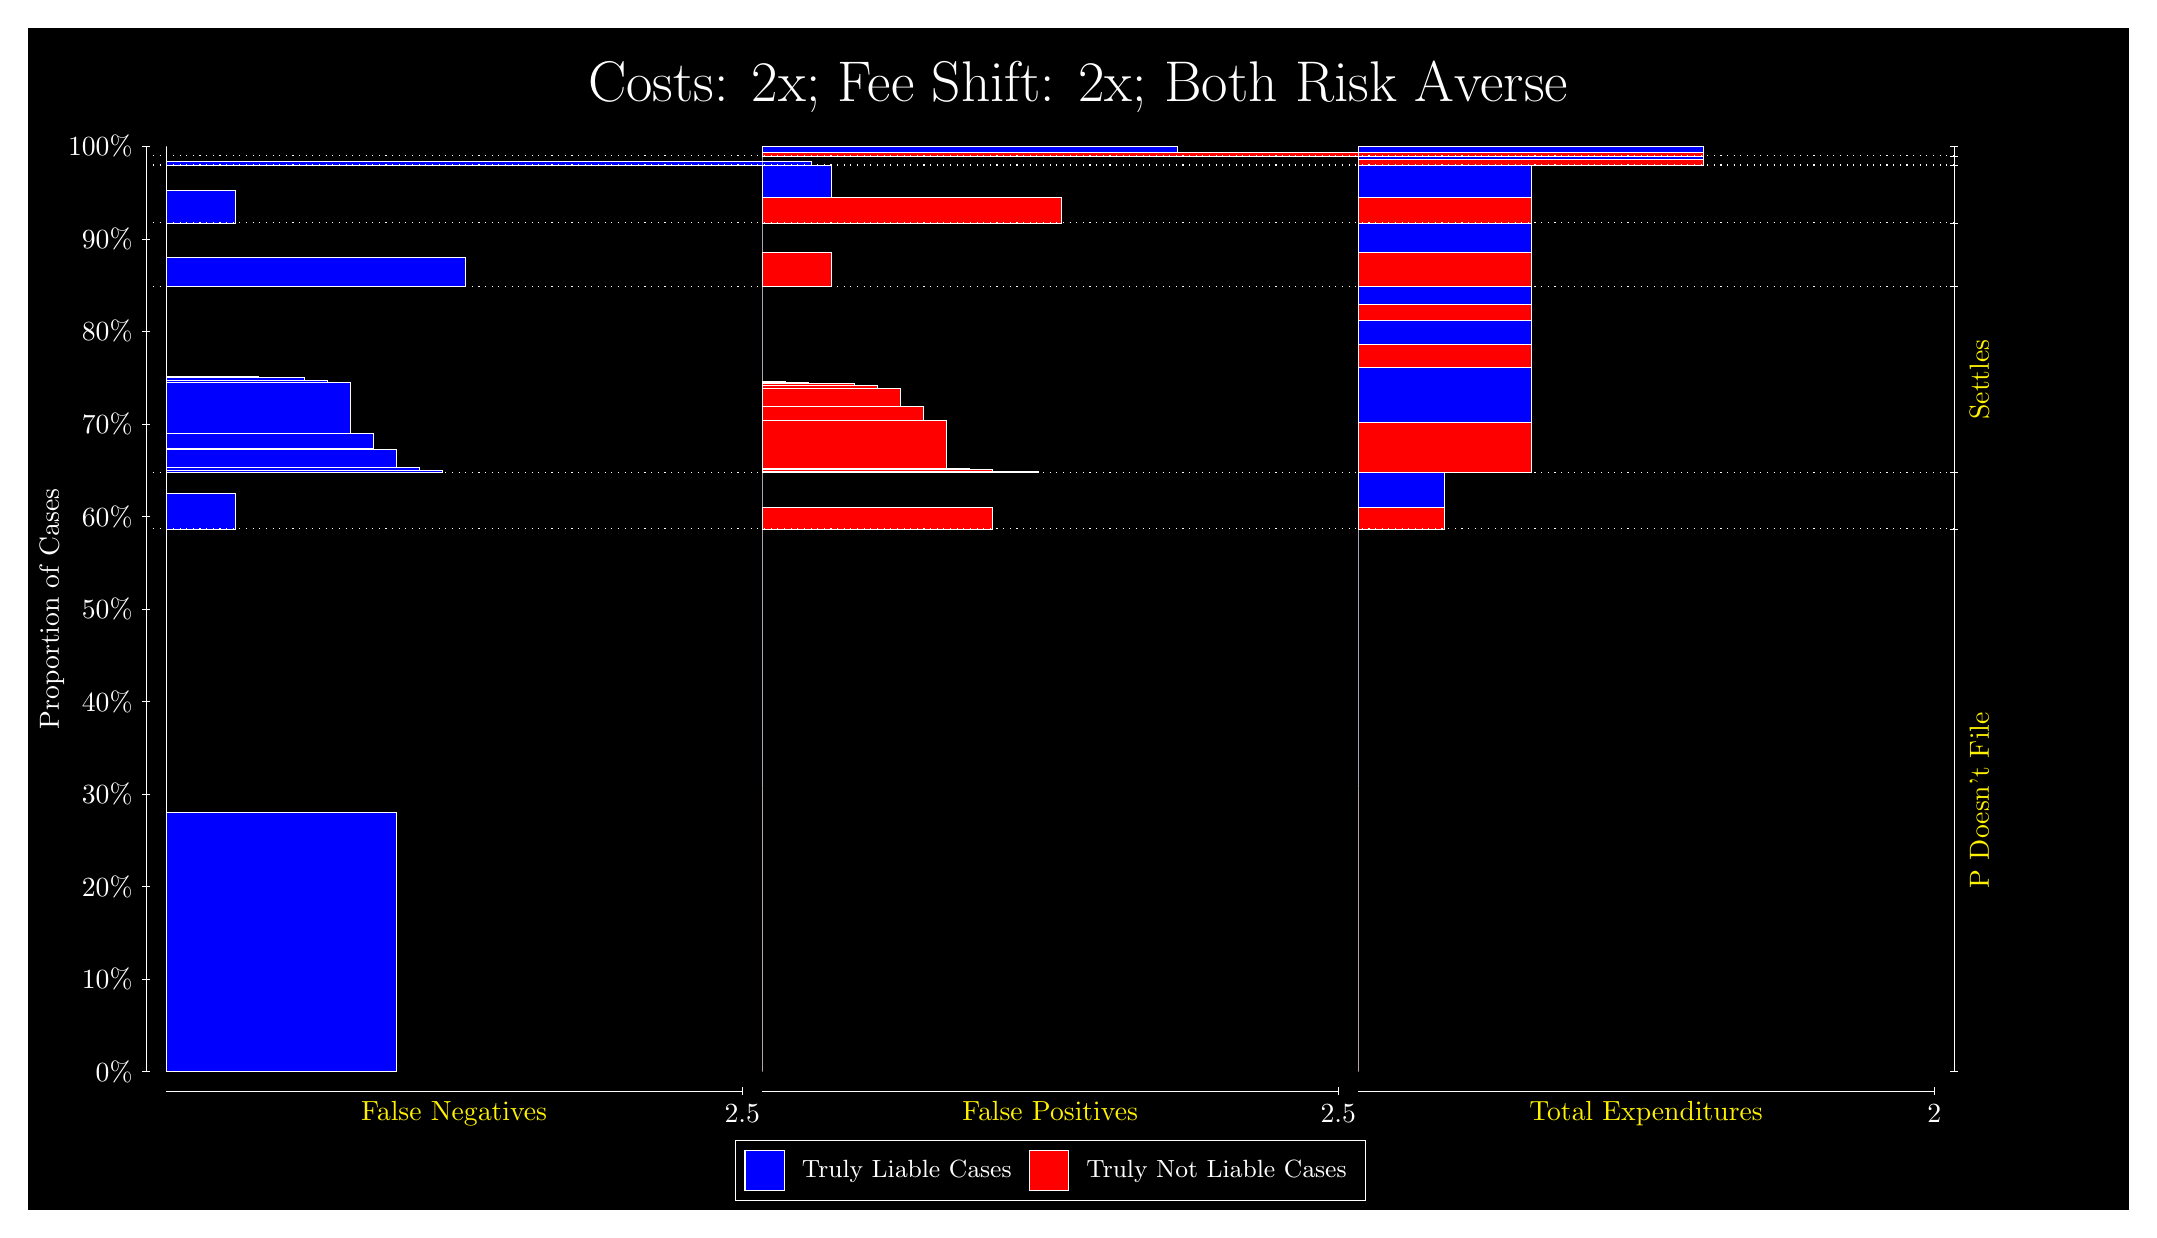
\begin{tikzpicture}
\draw[fill=black] (0,0) rectangle (26.667,15);
\draw[text=white] (0,13.5) rectangle (26.667,15) node[midway] {\huge Costs: 2x; Fee Shift: 2x; Both Risk Averse};
\draw[white, very thin] (1.5,1.75) -- (1.5,13.5);
\node[rotate=90, text=white, anchor=center] at (0.3, 7.625) {Proportion of Cases};
\draw[white, very thin] (1.45,1.75) -- (1.55,1.75);
\node[text=white, anchor=east] at (1.45, 1.75) {0\%};
\draw[white, very thin] (1.45,2.925) -- (1.55,2.925);
\node[text=white, anchor=east] at (1.45, 2.925) {10\%};
\draw[white, very thin] (1.45,4.1) -- (1.55,4.1);
\node[text=white, anchor=east] at (1.45, 4.1) {20\%};
\draw[white, very thin] (1.45,5.275) -- (1.55,5.275);
\node[text=white, anchor=east] at (1.45, 5.275) {30\%};
\draw[white, very thin] (1.45,6.45) -- (1.55,6.45);
\node[text=white, anchor=east] at (1.45, 6.45) {40\%};
\draw[white, very thin] (1.45,7.625) -- (1.55,7.625);
\node[text=white, anchor=east] at (1.45, 7.625) {50\%};
\draw[white, very thin] (1.45,8.8) -- (1.55,8.8);
\node[text=white, anchor=east] at (1.45, 8.8) {60\%};
\draw[white, very thin] (1.45,9.975) -- (1.55,9.975);
\node[text=white, anchor=east] at (1.45, 9.975) {70\%};
\draw[white, very thin] (1.45,11.15) -- (1.55,11.15);
\node[text=white, anchor=east] at (1.45, 11.15) {80\%};
\draw[white, very thin] (1.45,12.325) -- (1.55,12.325);
\node[text=white, anchor=east] at (1.45, 12.325) {90\%};
\draw[white, very thin] (1.45,13.5) -- (1.55,13.5);
\node[text=white, anchor=east] at (1.45, 13.5) {100\%};

\draw[white, very thin] (24.457,1.75) -- (24.457,13.5);
\draw[white, very thin] (24.407,1.75) -- (24.507,1.75);
\node[anchor=west] at (24.407, 1.75) {};
\draw[white, very thin] (24.407,8.6428) -- (24.507,8.6428);
\node[anchor=west] at (24.407, 8.6428) {};
\draw[white, very thin] (24.407,9.3615) -- (24.507,9.3615);
\node[anchor=west] at (24.407, 9.3615) {};
\draw[white, very thin] (24.407,11.718) -- (24.507,11.718);
\node[anchor=west] at (24.407, 11.718) {};
\draw[white, very thin] (24.407,12.527) -- (24.507,12.527);
\node[anchor=west] at (24.407, 12.527) {};
\draw[white, very thin] (24.407,13.263) -- (24.507,13.263);
\node[anchor=west] at (24.407, 13.263) {};
\draw[white, very thin] (24.407,13.378) -- (24.507,13.378);
\node[anchor=west] at (24.407, 13.378) {};
\draw[white, very thin] (24.407,13.5) -- (24.507,13.5);
\node[anchor=west] at (24.407, 13.5) {};

\draw[white, very thin, fill=blue] (1.75,1.75) rectangle (4.6775,5.0462);
\draw[white, very thin, fill=red] (1.75,5.0462) rectangle (1.75,8.6428);
\draw[white, very thin, fill=blue] (1.75,8.6428) rectangle (2.6283,9.0926);
\draw[white, very thin, fill=red] (1.75,9.0926) rectangle (1.75,9.3615);
\draw[white, very thin, fill=blue] (1.75,9.3615) rectangle (5.2631,9.3881);
\draw[white, very thin, fill=blue] (1.75,9.3881) rectangle (4.9703,9.4257);
\draw[white, very thin, fill=blue] (1.75,9.4257) rectangle (4.6775,9.6561);
\draw[white, very thin, fill=blue] (1.75,9.6561) rectangle (4.3848,9.6621);
\draw[white, very thin, fill=blue] (1.75,9.6621) rectangle (4.3848,9.8549);
\draw[white, very thin, fill=blue] (1.75,9.8549) rectangle (4.092,10.509);
\draw[white, very thin, fill=blue] (1.75,10.509) rectangle (3.7993,10.534);
\draw[white, very thin, fill=blue] (1.75,10.534) rectangle (3.5065,10.563);
\draw[white, very thin, fill=blue] (1.75,10.563) rectangle (3.2138,10.573);
\draw[white, very thin, fill=blue] (1.75,10.573) rectangle (2.921,10.583);
\draw[white, very thin, fill=red] (1.75,10.583) rectangle (1.75,11.718);
\draw[white, very thin, fill=blue] (1.75,11.718) rectangle (5.5558,12.093);
\draw[white, very thin, fill=red] (1.75,12.093) rectangle (1.75,12.527);
\draw[white, very thin, fill=blue] (1.75,12.527) rectangle (2.6283,12.939);
\draw[white, very thin, fill=red] (1.75,12.939) rectangle (1.75,13.263);
\draw[white, very thin, fill=blue] (1.75,13.263) rectangle (9.9471,13.308);
\draw[white, very thin, fill=red] (1.75,13.308) rectangle (1.75,13.378);
\draw[white, very thin, fill=red] (1.75,13.378) rectangle (1.75,13.425);
\draw[white, very thin, fill=blue] (1.75,13.425) rectangle (1.75,13.5);
\draw[white, very thin, fill=red] (9.3189,1.75) rectangle (9.3189,5.3466);
\draw[white, very thin, fill=blue] (9.3189,5.3466) rectangle (9.3189,8.6428);
\draw[white, very thin, fill=red] (9.3189,8.6428) rectangle (12.246,8.9118);
\draw[white, very thin, fill=blue] (9.3189,8.9118) rectangle (9.3189,9.3615);
\draw[white, very thin, fill=red] (9.3189,9.3615) rectangle (12.832,9.368);
\draw[white, very thin, fill=red] (9.3189,9.368) rectangle (12.539,9.3739);
\draw[white, very thin, fill=red] (9.3189,9.3739) rectangle (12.246,9.3941);
\draw[white, very thin, fill=red] (9.3189,9.3941) rectangle (11.954,9.4121);
\draw[white, very thin, fill=red] (9.3189,9.4121) rectangle (11.661,10.021);
\draw[white, very thin, fill=red] (9.3189,10.021) rectangle (11.368,10.201);
\draw[white, very thin, fill=red] (9.3189,10.201) rectangle (11.075,10.422);
\draw[white, very thin, fill=red] (9.3189,10.422) rectangle (10.783,10.468);
\draw[white, very thin, fill=red] (9.3189,10.468) rectangle (10.49,10.497);
\draw[white, very thin, fill=blue] (9.3189,10.497) rectangle (9.9044,10.507);
\draw[white, very thin, fill=blue] (9.3189,10.507) rectangle (9.6116,10.516);
\draw[white, very thin, fill=blue] (9.3189,10.516) rectangle (9.3189,11.718);
\draw[white, very thin, fill=red] (9.3189,11.718) rectangle (10.197,12.152);
\draw[white, very thin, fill=blue] (9.3189,12.152) rectangle (9.3189,12.527);
\draw[white, very thin, fill=red] (9.3189,12.527) rectangle (13.125,12.851);
\draw[white, very thin, fill=blue] (9.3189,12.851) rectangle (10.197,13.263);
\draw[white, very thin, fill=red] (9.3189,13.263) rectangle (9.3189,13.333);
\draw[white, very thin, fill=blue] (9.3189,13.333) rectangle (9.3189,13.378);
\draw[white, very thin, fill=red] (9.3189,13.378) rectangle (17.516,13.425);
\draw[white, very thin, fill=blue] (9.3189,13.425) rectangle (14.588,13.5);
\draw[white, very thin, fill=red] (16.888,1.75) rectangle (16.888,5.3466);
\draw[white, very thin, fill=blue] (16.888,5.3466) rectangle (16.888,8.6428);
\draw[white, very thin, fill=red] (16.888,8.6428) rectangle (17.986,8.9118);
\draw[white, very thin, fill=blue] (16.888,8.9118) rectangle (17.986,9.3615);
\draw[white, very thin, fill=red] (16.888,9.3615) rectangle (19.083,9.9965);
\draw[white, very thin, fill=blue] (16.888,9.9965) rectangle (19.083,10.689);
\draw[white, very thin, fill=red] (16.888,10.689) rectangle (19.083,10.989);
\draw[white, very thin, fill=blue] (16.888,10.989) rectangle (19.083,11.29);
\draw[white, very thin, fill=red] (16.888,11.29) rectangle (19.083,11.49);
\draw[white, very thin, fill=blue] (16.888,11.49) rectangle (19.083,11.718);
\draw[white, very thin, fill=red] (16.888,11.718) rectangle (19.083,12.152);
\draw[white, very thin, fill=blue] (16.888,12.152) rectangle (19.083,12.527);
\draw[white, very thin, fill=red] (16.888,12.527) rectangle (19.083,12.851);
\draw[white, very thin, fill=blue] (16.888,12.851) rectangle (19.083,13.263);
\draw[white, very thin, fill=red] (16.888,13.263) rectangle (21.279,13.333);
\draw[white, very thin, fill=blue] (16.888,13.333) rectangle (21.279,13.378);
\draw[white, very thin, fill=red] (16.888,13.378) rectangle (21.279,13.425);
\draw[white, very thin, fill=blue] (16.888,13.425) rectangle (21.279,13.5);
\draw[white, dotted] (1.5,8.6428) -- (24.457,8.6428);
\draw[white, dotted] (1.5,9.3615) -- (24.457,9.3615);
\draw[white, dotted] (1.5,11.718) -- (24.457,11.718);
\draw[white, dotted] (1.5,12.527) -- (24.457,12.527);
\draw[white, dotted] (1.5,13.263) -- (24.457,13.263);
\draw[white, dotted] (1.5,13.378) -- (24.457,13.378);
\draw[white, very thin] (1.75,1.5) -- (9.0689,1.5);
\node[text=yellow, anchor=north] at (5.4094, 1.5) {False Negatives};
\draw[white, very thin] (9.0689,1.45) -- (9.0689,1.55);
\node[text=white, anchor=north] at (9.0689, 1.45) {2.5};

\draw[white, very thin] (9.3189,1.5) -- (16.638,1.5);
\node[text=yellow, anchor=north] at (12.978, 1.5) {False Positives};
\draw[white, very thin] (16.638,1.45) -- (16.638,1.55);
\node[text=white, anchor=north] at (16.638, 1.45) {2.5};

\draw[white, very thin] (16.888,1.5) -- (24.207,1.5);
\node[text=yellow, anchor=north] at (20.547, 1.5) {Total Expenditures};
\draw[white, very thin] (24.207,1.45) -- (24.207,1.55);
\node[text=white, anchor=north] at (24.207, 1.45) {2};

\node[text=yellow, centered, rotate=90] at (24.777, 5.1964) {P Doesn't File};

\node[text=yellow, centered, rotate=90] at (24.777, 10.54) {Settles};





\draw (12.978300999999998,1.5) node[draw=none] (baseCoordinate) {};
\begin{scope}[align=center]
        \matrix[scale=0.5, draw=white, below=0.5cm of baseCoordinate, nodes={draw}, column sep=0.1cm]{
            \node[rectangle, draw, minimum width=0.5cm, minimum height=0.5cm, fill=blue] {}; &
            \node[draw=none, font=\small, text=white] (B) {Truly Liable Cases}; &
            \node[rectangle, draw, minimum width=0.5cm, minimum height=0.5cm, fill=red] {}; &
            \node[draw=none, font=\small, text=white] (B) {Truly Not Liable Cases}; \\
            };
\end{scope}

\end{tikzpicture}
\end{document}